\newSec[Arch]{Software-Architektur}{1}
In diesem Kapitel soll die Architektur des Projekts umrissen werden. 


\newSec[ArchConcept]{Architektur Konzept}{2}
Der Aufbau der Architektur entspricht den Konzept der \clean. Diesem Prinzip folgend zeigen sämtliche Abhängigkeiten des Codes auf \textit{weiter innen liegende} Schichten.
Die Farbgebung in \refImg{fig:Packs} orientiert sich an den Inhalten der Vorlesung \texttt{Advanced Software-Engineering} der \DHBW\footnote{An dieser Stelle sei darauf hingewiesen, dass \refImg{fig:Packs} in der Ausarbeitung für die genannte Vorlesung auftaucht.}.

\begin{figure}[ht!]
\vspace{0.25cm}
\begin{center}
\fbox{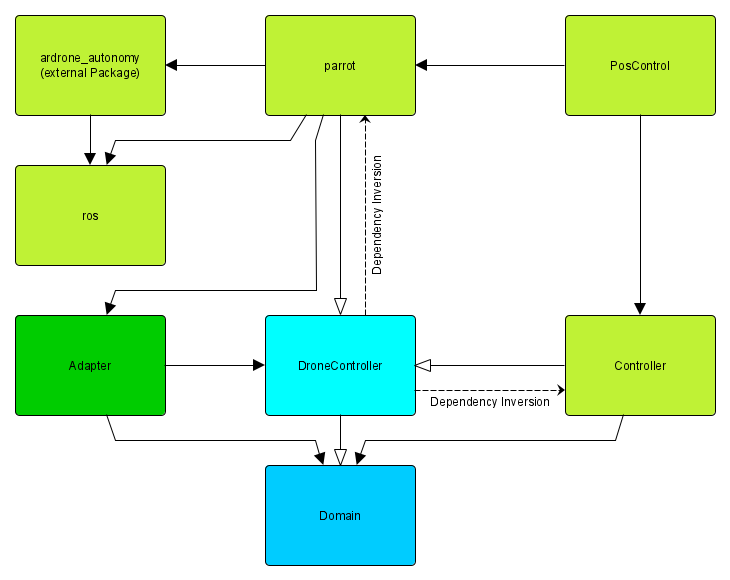
\includegraphics[width=15cm]{Pictures/Architecture Blocks.png}}
\caption{Architektur des Regelungssystems}
\label{fig:Packs}
\end{center}

\vspace{0.25cm}
\refImgShort{fig:Packs} zeigt das Konzept der Architektur. Die Bedeutungen der Pfeile orientieren sich an UML-Klassendiagrammen. Die Farbgebung unterscheidet die verschiedenen Schichten der \clean: \textit{Domain-Layer} (blau), \textit{Application-Layer} (hellblau), \textit{Adapter-Layer} (grün), \textit{PlugIn-Layer} (hellgrün).
\end{figure}



\newSec[ArchDomain]{\textit{Domain} \Pack}{2}
Im \textit{Domain} \Pack\ sind grundlegende Klassen abgelegt. Diese werden von den nachfolgend beschriebenen Schichten eingebunden. Gemeinsam mit dem \textit{DroneController} \Pack\ bildet es das Herzstück der Anwendung. Eine eindeutige Zuordnung der Klassen in diese beiden \Pack[s] ist diskutabel.


\newSec[ArchDrone]{\textit{DroneController} \Pack}{2}
Das Entwurfsmuster des \textit{Application-Layer} entspricht einer \textit{Bridge}. Ziel ist es, sowohl die eingesetzte Drohne, als auch die Implementierung des Reglers mit überschaubarem Aufwand austauschen zu können.

Hierin werden die grundlegenden Aufgaben für die Regelung einer Drohne übernommen. Eine detalliertere Beschreibung findet sich im Kapitel \refCap{ImplApp}.


\newSec[ArchAdapter]{\textit{Adapter} \Pack}{2}
Im \textit{Adapter} \Pack\ wird die Signalverarbeitung der Rohdaten übernommen und anschließend in einem aktuellen Zustand zur Weiteren Verarbeitung bereitgestellt.


\newSec[ArchController]{\textit{Controller} \Pack}{2}
Das \textit{Controller} \Pack\ einspricht beinhaltet Regelungsglieder, welche für eine beliebige Regelung im Allgemeinen genutzt werden können. Die Interaktion wird durch die Fassade \CodeClass{PoseController} an das Aufgabenfeld dieser \Arbeit\ angepasst.


\newSec[ArchParrot]{\textit{parrot} \Pack}{2}
Die Interaktion mit der in dieser \Arbeit\ eingesetzten Hardware wird vom gleichnamigen \textit{parrot} \Pack\ übernommen. Hier sind verschiedene Klassen enthalten, welche mittels \ROS\ \Topic[s] mit der Drohne kommunizieren und sowie Messdaten von der Drohne zur Verarbeitung bereitstellen, sowie Steuerungsbefehle an die Drohne übersenden.


\newSec[ArchPosControl]{\textit{PosControl} \Pack}{2}
Das \textit{PosControl} \Pack\ kann als Dach-Software angesehen werden. hierin wird die \CodeMeth{main()}-Methode aufgerufen und die übergeordnete verwaltende Klasse initialisiert.
